\documentclass{article}


% if you need to pass options to natbib, use, e.g.:
%     \PassOptionsToPackage{numbers, compress}{natbib}
% before loading neurips_2022


% ready for submission
\usepackage[final]{neurips_2022}
\usepackage{multirow}
\usepackage[final]{graphicx}


% to compile a preprint version, e.g., for submission to arXiv, add add the
% [preprint] option:
%     \usepackage[preprint]{neurips_2022}


% to compile a camera-ready version, add the [final] option, e.g.:
%     \usepackage[final]{neurips_2022}


% to avoid loading the natbib package, add option nonatbib:
%    \usepackage[nonatbib]{neurips_2022}


\usepackage[utf8]{inputenc} % allow utf-8 input
\usepackage[T1]{fontenc}    % use 8-bit T1 fonts
\usepackage{hyperref}       % hyperlinks
\usepackage{url}            % simple URL typesetting
\usepackage{booktabs}       % professional-quality tables
\usepackage{amsfonts}       % blackboard math symbols
\usepackage{nicefrac}       % compact symbols for 1/2, etc.
\usepackage{microtype}      % microtypography
\usepackage{xcolor}         % colors


\title{Project: Learning Based RRT using a Visual Classifier as a Cost Function}


% The \author macro works with any number of authors. There are two commands
% used to separate the names and addresses of multiple authors: \And and \AND.
%
% Using \And between authors leaves it to LaTeX to determine where to break the
% lines. Using \AND forces a line break at that point. So, if LaTeX puts 3 of 4
% authors names on the first line, and the last on the second line, try using
% \AND instead of \And before the third author name.

\author{Aaron Kampmeier \\ \texttt{akampmei@asu.edu} \And Brandon Evans \\ \texttt{bpevans@asu.edu} \And Braeden Woodard \\ \texttt{bmwoodar@asu.edu} \And Pavan Kumar Raja \\ \texttt{praja3@asu.edu}}

  % examples of more authors
  % \And
  % Coauthor \\
  % Affiliation \\
  % Address \\
  % \texttt{email} \\
  % \AND
  % Coauthor \\
  % Affiliation \\
  % Address \\
  % \texttt{email} \\
  % \And
  % Coauthor \\
  % Affiliation \\
  % Address \\
  % \texttt{email} \\
  % \And
  % Coauthor \\
  % Affiliation \\
  % Address \\
  % \texttt{email} \\



\begin{document}

% To cite something use \cite{} command such as:
% \cite{Zuo}
% \cite{Perez}


\maketitle

% \begin{abstract}
% % TODO Evaluate if we need an abstract, probably would be good to have
% In robotic navigation and exploration, there is a need to investigate efficent methods to handle continous state and control spaces. Many contributions have proposed variations of RRT algorithms that can more efficiently handle these enviroments over an Markov Decision Process (MDP). In this paper, we propose a method that expands on a proposed RRT variant that incorporates behvior cloning (BC) and utilizes a visual classifier to learn the cost function of the optimal trajectories. 
% \end{abstract}

\section{Introduction}

Rapidly-Exploring Random Trees (RRT) \cite{Steven} have proven to be a very useful sample-based path-planning algorithm to efficiently search high-dimensional spaces. However, RRT can be hindered in environments with obstacles or specific pathways to a goal. The algorithm may waste time exploring down irrelevant or blocked paths. In this paper, we will survey various learning approaches to problems encountered by RRT in such environments, evaluate a baseline modified RRT algorithm based on behavior cloning, present the results of our Visual Classifier assisted RRT algorithm, and discuss our future work. 

\section{Problem Statement}

% TODO Finish problem statement
A basic RRT algorithm's performance can suffer in configuration spaces with obstacles by exploring down irrelevant or blocked paths. The surveyed learning improvements to RRT may help but they still need a way to discover where the goal states and relevant obstacles are in relation to the agent. This problem can arise a variety of different domains such as expansions through mazes, robotic control in constrained spaces \cite{9164659}, and systems testing of multi-step processes \cite{Zuo}. There exists previous work regarding trying to solve this problem via RRT algorithms that use Behavior Cloning to seed the RRT tree. This paper uses one of these algorithms, CA-RRT\cite{Zuo}. as a baseline and aims to develop a BC RRT algorithm that uses a visual classifier to guide RRT expansion.


\section{Related Work}

In the last few years, several contributions to robotic navigation and exploration have been proposed that incorporate variations of sampling-based costmap planners, such as RRT or RRT*, and learning from demonstrations. Zuo et. al. \cite{Zuo} proposes a method, Clone Assisted RRT (CA-RRT), that learns heuristics for a search-based algorithm from a limited number of human demonstrations. CA-RRT is an expansion of the human-seeded RRT (HS-RRT) proposed by Chang et. al. \cite{Chang}, which uses states from human demonstrations as seed configurations states within an RRT. This expansion includes adding a first-person image-state-based (behavioral) cloning approach over the HS-RRT. Zuo et. al. \cite{Zuo} method consists of collecting a set of human-created trajectories and training a behavioral cloning policy using the first-person state-action pairs from those trajectories to seed the RRT. These heuristics allow the search algorithms to automatically test other states in the game thus removing the necessity to test all possible scenarios in the game through human game play.

Perez et. al. \cite{Perez} also proposes an approach to learn navigation behaviors from demonstrations with the use of sampling-based costmap planners, though they propose the use Inverse Reinforcement Learning (IRL) concepts to identify the RRT cost function that best fits the example trajectories. The proposed method, Rapidly-exploring random Trees Inverse Reinforcement Learning (RTIRL), makes use of the RRT* instead of a Markov Decision Process (MDP). This is due to the advantages that RRT* has over MDP, in which RRT* can handle continuous state and control spaces. Perez et. al. \cite{Perez} RTIRL method is used to extract the proper weights of the cost function from demonstration trajectories, which can then be used later in the RRT* process to allow the robot to reproduce the desired behavior at various scenarios. 

Both papers propose learning algorithms that use sampling-based costmap planners for path planning and exploration. Our proposed method will also be expanding upon the RRT algorithm and involve collecting and utilizing human demonstrations to allow for learning from demonstrations. Our proposed algorithm will incorporate a similar behavior cloning (BC) approach to that of Zuo et. al. \cite{Zuo} as the BC policy will be act as a seed in the initial RRT configuration. In addition to BC, we aim to use a visual classifier to learn a cost function, by using an image to gather samples from various locations to determine the cost to reach the goal state. This approach is a development of and similar to the work by Majeed et al., who successfully used an image pre-processor to locate objects in an environment prior to performing path planning utilizing an A* algorithm. \cite{Majeed} They found that using an image processor to locate obstacles in combination with A* planning was successful in path finding in both static and dynamic environments. \cite{Majeed} We aim to further expand on this paper's work by implementing image processing into the cost function of RRT rather than pre-processing. We aim to train a behavior cloning policy on a 2D image of the environment, similar to the greyscale 2D images used in the paper by Majeed et al. as our image also uses high contrast to aid in the performance of our algorithm. 


\section{Problem Domain}

The problem domain consists of 2D pygame environment which contains obstacles that create a maze that an agent must navigate to reach a goal location. 
The background of this environment is black, the obstacles are blue, the agent is red, and the goal is green to enhance contrast. The start location, goal location, and obstacles can either be static or dynamic across instances of the game depending on user arguments.

% TODO: Reword the followings, add description of discrete action space
For our problem the agent is creating a path to navigate from start to goal. In order to do this, our agent uses a variety RRT algorithms.

Out agent is tested in a both static and dynamic 500x800 pixel environments using either basic RRT, BCRRT, or Image BCRRT. BCRRT is our baseline, and Image BCRRT is our visual classifier assisted BCRRT. For the Image BCRRT the input to the agent is a 2D image of the environment with the action the agent is taking in that state.

\section{Learning Baseline}

In this paper we will show results relative to some baseline. The baseline we decided to work off of is a trained implementation of the CA-RRT algorithm \cite{Zuo} that we call BCRRT. 
BCRRT works by first rolling out a trained Behavior Cloning policy to generate a path. 
This path is then used to seed a standard RRT algorithm. The idea is that the path rolled out by the BC model will guide the RRT expansion. 

To keep complexity low for the baseline, we used a environment where the goal state and the obstacles are kept static. The state space is the agent's and the goal's current coordinates in the maze environment.
Table \ref{bcrrt model summary} shows the neural network model used for the BCRRT algorithm. This model was trained with around 20,000 demonstrations. 

\begin{table}[h]
\parbox{.45\linewidth}{
  \caption{BCRRT Model Summary}
  \label{bcrrt model summary}
  \centering
  \begin{tabular}{lll}
    \cmidrule(r){1-3}
   Layer (Type)          & Output Shape       &Parameter count\\
    \midrule
    Linear-1 & [-1, 8] & 40\\
    ReLU-2 & [-1, 8] & 0\\
    BatchNorm1d-3 & [-1, 8] & 16\\
    Linear-4 & [-1, 8] & 72\\
    ReLU-5 & [-1, 8] & 0\\
    BatchNorm1d-6 & [-1, 8] & 16\\
    Linear-7 & [-1, 4] & 36\\
    ReLU-8 & [-1, 4] & 0\\
    BatchNorm1d-9 & [-1, 4] & 8\\
    Linear-10 & [-1, 4] & 20\\
    ReLU-11 & [-1, 4] & 0\\
    BatchNorm1d-12 & [-1, 4] & 8\\
    \bottomrule
    \cmidrule(r){1-2}
        Total Parameters & & 216\\
    \bottomrule
  \end{tabular}}
  \hfill
\parbox{.45\linewidth}{
\caption{IMGBCRRT Model Summary}
	\label{imgbcrrt model summary}
	\centering
	\begin{tabular}{lll}
		\cmidrule(r){1-2}
		Layer (Type) & Output Shape\\
		\midrule
		Resize & [3,256,256]\\
		ConvertImageToFloat & [3,256,256]\\
		Normalize & [3,256,256]\\
		\midrule
		Conv2d & [64,127,127]\\
		ReLU & --\\
		MaxPool2d & [64,63,63]\\
		Conv2d & [128,31,31]\\
		ReLU & --\\
		MaxPool2d & [128,15,15]\\
		InstanceNorm2d & --\\
		\midrule
		Flatten & 28800\\
		Linear & 64\\
		ReLU & 64\\
		Linear & 4\\
		ReLU & 4\\
		\bottomrule
	\end{tabular}
	}
\end{table}

\section{IMGBCRRT - Novel Model}

We now introduce a novel model called IMGBCRRT that works off of the same concepts as BCRRT but where the state space is a 2D image of the entire game field (as opposed to just the coordinates of objects). 
Table \ref{imgbcrrt model summary} shows the structure of the IMGBCRRT Convolutional Neural Network. It first performs some preprocessing on an input image that normalizes and scales all images down to size 256x256. Then the image is passed through 2 convolutional and pooling layers. Finally the input is flattened and passed through 2 fully connected layers to obtain 4 outputs that correspond to the 4 potential actions.

We trained this model under 3 different scenarios: static start/goal/obstacles, static start/goal + dynamic obstacles, static goal + dynamic start/obstacles. Each training used an autogenerated dataset of about 10,000 labeled images. 
To further validate our following results, we also trained a dynamic start/obstacles + static goal model twice more on datasets of size 20,000 and 100,000. The classification accuracy when evaluating every model after training was always around 48\%.

% Detail experiment metrics BW
\section{Experiment Metrics}

The metrics being evaluated in the experiment include the following:
\begin{itemize}
	\item{Success Rate: The percentage of successes that the agent successfully reaches the goal.}
	\item{Time: The time taken by the agent from the start of RRT to the terminal node or condition i.e. when the limit of 1000 expansions is met.}
	\item{Number of Expansions: The number of nodes in the RRT graph at termination.}
\end{itemize}

\section{Experiment Results}
% Detail result findings BW
As our goal was to develop a RRT algorithm that uses a visual classifier to learn a cost function. The baseline used for this paper required a learning-based approach, as such, we decided to utilize CARRT as our baseline rather than a standard RRT. The above metrics were used for an initial evaluatation of both our baseline algorithm, which was a version of CA-RRT (BCRRT), and a standard RRT algorithm. In order to ensure the baseline BCRRT was performing correctly, the metric results must reflect an improvement of BCRRT over the strandard RRT. The initial baseline results for BCRRT can be seen in Table \ref{BCRRT Results}, while the results for RRT are shown in Appendix A: Table \ref{RRT Metrics}. The experiment does not directly compare RRT with our proposed IMGBCRRT algorithm, as we are solely focusing on a learning-based approach. After training numerous models of IMGBCRRT, we proceeded with the experiment phase of this paper, this included the testing of our proposed algorithm. We performed testing on three different configurations of IMGBCRRT. The first configuration consisted of a static enviroment with static obstacles and static start/goal locations, which is labeled as IMGBCRRT SA, and is shown in Table \ref{IMGBCRRT SA Results}. The second configuration consisted of a mixed enviroment with dynamic obstacles and static start/goal locations, which is labeled as IMGBCRRT SDO, and is shown in Table \ref{IMGBCRRT SDO Results}. The last configuration consisted of a dynamic enviroment with dynamic obstacles and dynamic start/goal locations, which is labeled as IMGBCRRT DA, and is shown in Table \ref{IMGBCRRT DA Results}. 

To properly evaluate the performance of IMGBCRRT, the experiment consisted of testing the three configurations of IMGBCRRT against the baseline BCRRT. The BCRRT configuration consisted of a static enviroment with static obstacles and static start/goal locations. The experiment was done over five iterations with the results of the metrics being collected during each iteration of the test. The mean and standard deviation of the metric results are provided in each results table as well as a box and whisker plot. The results of the baseline BCRRT compared to RRT reflect an expected outcome of  BCRRT performing better overall than the RRT algorithm. The RRTprovides a mean success rate of .79, a mean time of 3.39 s $\pm$ 1.20 s, and a mean expansions of 744.48 $\pm$ 208.45. While the BCRRT provides a mean success rate of .90, a mean time of 1.94 s $\pm$ 1.73 s, and a mean number of expansions of 436.48 $\pm$ 375.33.

In regard to the results of the direct comparison of BCRRT and IMGBCRRT SA, we can see a significant improvement on all metrics. The results show a significant reduction of time with IMGBCRRT SA with a mean time of .92 s $\pm$ .31 s and a mean number of expansions of 22.09 $\pm$ 84.50. The evaluation of the two remaining configurations of IMGBCRRT in comparison to IMGBCRRT SA reflect an increase of mean time and number of expansions when dynamic obstacles are used though the success rate remains at ~.90. We can see from the results that the standard deviation (SD) seems rather large, this may be due to the small number of iterations that were used in testing, this can be addressed in future work by performing testing with a larger number of iterations. Due to the large SD values, we further analyzed the data by calculating the coefficient of variation (CV) for each of the results to determine the level of dispersion around the mean, shown in Appendix A: Table \ref{CV}. Despite the large standard deviations seen in the results, we see a reasonable dispersion of mean time and number of expansions (with the exception of IMGBCRRT SA). 

%  Updated and Correct Tables BW
\begin{table}[h]
  \caption{Results from BCRRT Algorithm}
  \label{BCRRT Results}
  \centering
  \begin{tabular}{llllll}
    \cmidrule(r){1-6}
   Iteration & Success Rate & Mean Time(s) & Std. Dev Time & Mean Expansions & Std. Dev Expansions\\
    \midrule
    1 & .89 & 1.9586 & 1.8819 & 440.6875 & 378.6503 \\
    2 & .91 & 2.0340 & 1.7459 & 442.09 & 372.4981 \\
    3 & .92 & 1.6560 & 1.4974 & 439.7563 & 375.8521 \\
    4 & .90 & 2.0366 & 1.8273 & 428.4387 & 376.2023 \\
    5 & .89 & 2.0287 & 1.6985 & 431.4369 & 373.4285 \\
 \midrule
  AVG & .902 & 1.9428 & 1.7302 & 436.4819 & 375.3263 \\
    \bottomrule
  \end{tabular}
\end{table}

\begin{table}[h]
  \caption{Results from IMGBCRRT SA Algorithm}
  \label{IMGBCRRT SA Results}
  \centering
  \begin{tabular}{llllll}
    \cmidrule(r){1-6}
   Iteration & Success Rate & Mean Time(s) & Std. Dev Time & Mean Expansions & Std. Dev Expansions\\
    \midrule
    1 & 1.0 & .8916 & .2051 & 19.8276 & 66.0555 \\
    2 & 1.0 & .8958 & .1310 & 18.4576 & 63.0348 \\
    3 & 1.0 & .8971 & .1238 & 16.7414 & 54.4690 \\
    4 & 1.0 & .9432 & .4144 & 25.1466 & 101.5863 \\
    5 & .98 & .9743 & .6745 & 30.3017 & 137.3698 \\
 \midrule
  AVG & .996 & .9204 & .3097 & 22.0950 & 84.5031 \\
    \bottomrule
  \end{tabular}
\end{table}

\begin{table}[h]
  \caption{Results from IMGBCRRT SDO Algorithm}
  \label{IMGBCRRT SDO Results}
  \centering
  \begin{tabular}{llllll}
    \cmidrule(r){1-6}
   Iteration & Success Rate & Mean Time(s) & Std. Dev Time & Mean Expansions & Std. Dev Expansions\\
    \midrule
    1 & 1.0 & 1.4602 & .8591 & 196.7556 & 194.4713 \\
    2 & .92 & 2.6790 & 1.8534 & 374.2079 & 313.2433 \\
    3 & .73 & 4.3425 & 1.8081 & 696.5349 & 293.5065 \\
    4 & .98 & 1.8653 & 1.6107 & 208.3444 & 290.2712 \\
    5 & .98 & 1.6502 & 1.0182 & 222.1038 & 249.5101 \\
 \midrule
  AVG & .922 & 2.3994 & 1.4299 & 339.5893 & 268.2005 \\
    \bottomrule
  \end{tabular}
\end{table}

\begin{table}[hbt!]
  \caption{Results from IMGBCRRT DA Algorithm}
  \label{IMGBCRRT DA Results}
  \centering
  \begin{tabular}{llllll}
    \cmidrule(r){1-6}
   Iteration & Success Rate & Mean Time(s) & Std. Dev Time & Mean Expansions & Std. Dev Expansions\\
    \midrule
    1 & .99 & 2.2373 & .7730 & 283.5508 & 181.8569 \\
    2 & .94 & 2.7234 & 1.1715 & 564.7465 & 246.4456 \\
    3 & .81 & 2.2974 & 1.4021 & 360.9149 & 378.8530 \\
    4 & .91 & 1.4934 & 1.0860 & 257.0303 & 303.3063 \\
    5 & .86 & 3.6526 & 1.2020 & 637.5954 & 264.6904 \\
 \midrule
  AVG & .9020 & 2.4808 & 1.1269 & 420.7676 & 275.0304 \\
    \bottomrule
  \end{tabular}
\end{table}

%  Update figures

\begin{figure}[h]
	\centering
\begin{minipage}{.5\textwidth}
\centering
	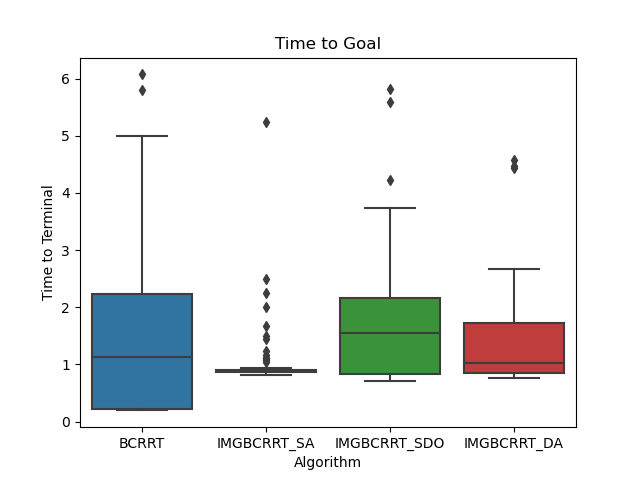
\includegraphics[width=.9\linewidth]{TTG1.png}
        \caption{Time to reach goal}
\end{minipage}%
\begin{minipage}{.5\textwidth}
\centering
	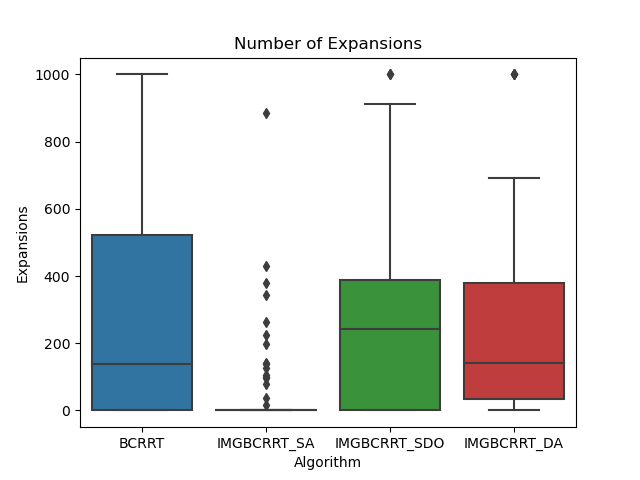
\includegraphics[width=.9\linewidth]{Expans1.png}
        \caption{Number of nodes expanded}
\end{minipage}

\end{figure}

\begin{figure}[h]
	%\centerline{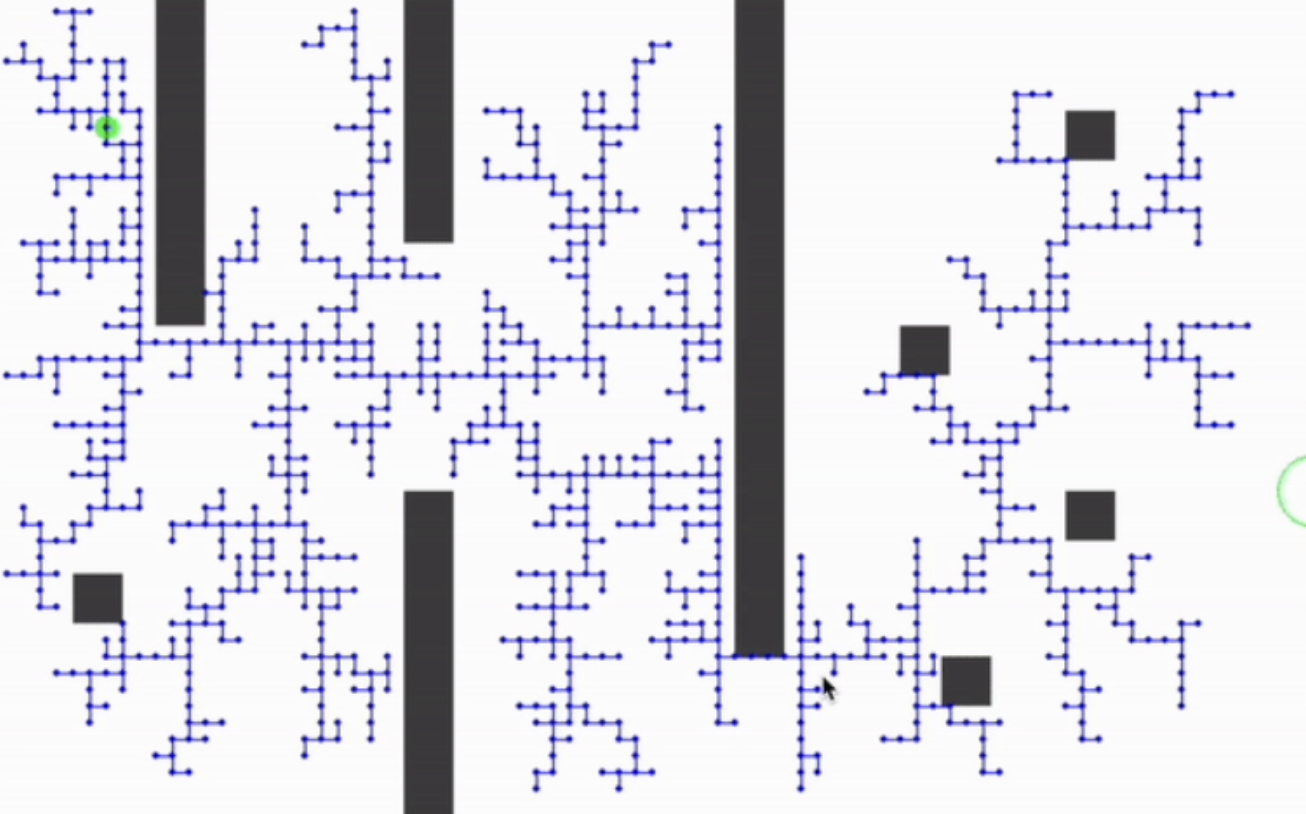
\includegraphics[scale=0.40]{RRT.png}}
        \caption{Expansion based solely on RRT}
\end{figure}

\begin{figure}[h]
	%\centerline{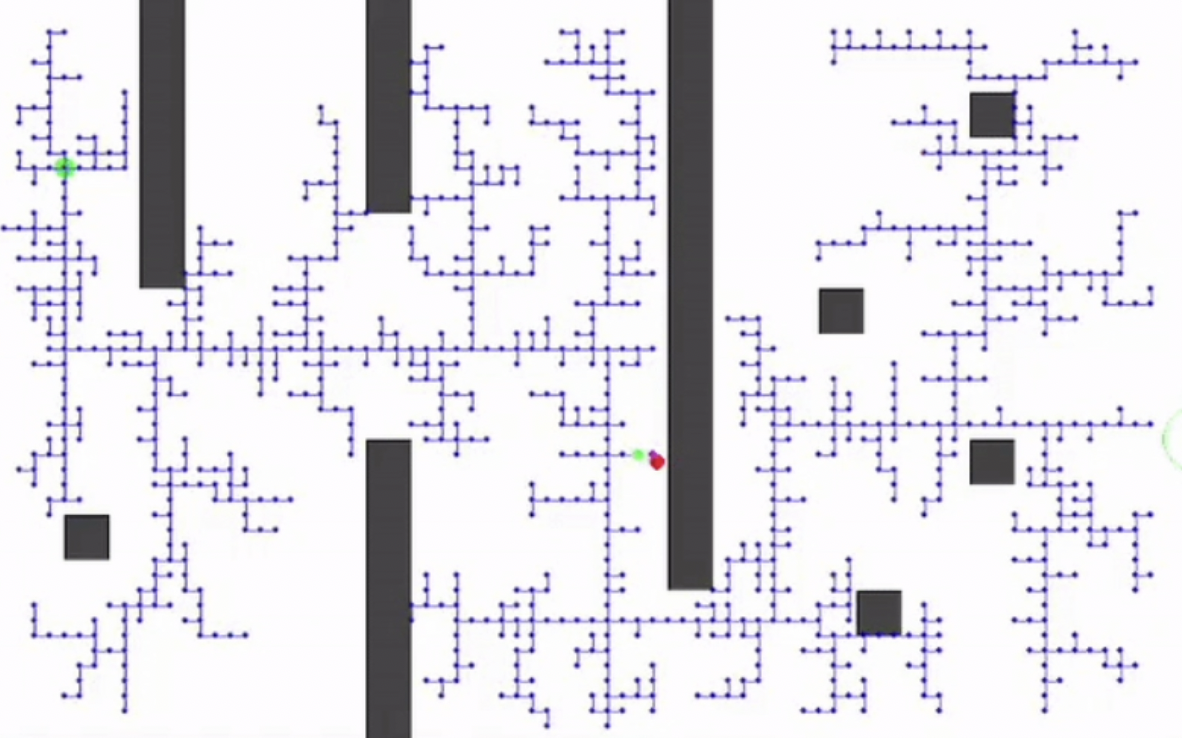
\includegraphics[scale=0.45]{BCRRT.png}}
        \caption{Expansion after behavior cloned roll-out}
\end{figure}

\vspace{1cm}
\section{Future Work}
Experimentations - 
\begin{itemize}
  \item Our system can be summarised as a model-free learning AI (where its trying to learn the domain to help RRT expansion). However, we feel the learning part is not agnostic because we have design it based on the problem domain.
  \item It would be interesting to see if embedding the action value into few training samples for CNN and trying to bias the network will help in getting better results. This is possible because our action/labels can be easily indicated by image/input.
\end{itemize}


\bibliographystyle{plain}
\bibliography{../sources.bib}

\vspace{1cm}
\section{Appendix A: Supplementary Material}

\begin{table}[h]
  \caption{Metrics from RRT Algorithm}
  \label{RRT Metrics}
  \centering
  \begin{tabular}{llllll}
    \cmidrule(r){1-6}
   Iteration & Success Rate & Mean Time(s) & Std. Dev Time & Mean Expansions & Std. Dev Expansions\\
    \midrule
    1 & .79 & 3.6179 & 1.2385 & 745.3562 & 211.5847 \\
    2 & .81 & 3.5861 & 1.1871 & 752.03 & 202.2828 \\
    3 & .79 & 2.9090 & 1.0498 & 751.5603 & 209.2586 \\
    4 & .77 & 3.4672 & 1.2880 & 734.6838 & 213.4561 \\
    5 & .79 & 3.3586 & 1.2298 & 738.7589 & 205.6531 \\
 \midrule
  AVG & .79 & 3.3878 & 1.1986 & 744.4778 & 208.4471 \\
    \bottomrule
  \end{tabular}
\end{table}

\begin{table}[h]
  \caption{Coefficient of Variation (CV)}
  \label{CV}
  \centering
  \begin{tabular}{llllll}
    \cmidrule(r){1-3}
   Algorithm  & CV Time(s) &  CV Expansions\\
    \midrule
    RRT & 0.3544 & .2800\\
    BCRRT & .8916 & .8600\\
    IMGBCRRT SA & .3292 & 3.7147\\
     IMGBCRRT SDO & .6354 & .9527\\
     IMGBCRRT DA  & .4884 & .7445\\
    \bottomrule
  \end{tabular}
\end{table}

%%%%%%%%%%%%%%%%%%%%%%%%%%%%%%%%%%%%%%%%

% \section{Submission of papers to NeurIPS 2022}


% Please read the instructions below carefully and follow them faithfully.


% \subsection{Style}


% Papers to be submitted to NeurIPS 2022 must be prepared according to the
% instructions presented here. Papers may only be up to {\bf nine} pages long,
% including figures. Additional pages \emph{containing only acknowledgments and
% references} are allowed. Papers that exceed the page limit will not be
% reviewed, or in any other way considered for presentation at the conference.


% The margins in 2022 are the same as those in 2007, which allow for $\sim$$15\%$
% more words in the paper compared to earlier years.


% Authors are required to use the NeurIPS \LaTeX{} style files obtainable at the
% NeurIPS website as indicated below. Please make sure you use the current files
% and not previous versions. Tweaking the style files may be grounds for
% rejection.


% \subsection{Retrieval of style files}


% The style files for NeurIPS and other conference information are available on
% the World Wide Web at
% \begin{center}
%   \url{http://www.neurips.cc/}
% \end{center}
% The file \verb+neurips_2022.pdf+ contains these instructions and illustrates the
% various formatting requirements your NeurIPS paper must satisfy.


% The only supported style file for NeurIPS 2022 is \verb+neurips_2022.sty+,
% rewritten for \LaTeXe{}.  \textbf{Previous style files for \LaTeX{} 2.09,
%   Microsoft Word, and RTF are no longer supported!}


% The \LaTeX{} style file contains three optional arguments: \verb+final+, which
% creates a camera-ready copy, \verb+preprint+, which creates a preprint for
% submission to, e.g., arXiv, and \verb+nonatbib+, which will not load the
% \verb+natbib+ package for you in case of package clash.


% \paragraph{Preprint option}
% If you wish to post a preprint of your work online, e.g., on arXiv, using the
% NeurIPS style, please use the \verb+preprint+ option. This will create a
% nonanonymized version of your work with the text ``Preprint. Work in progress.''
% in the footer. This version may be distributed as you see fit. Please \textbf{do
%   not} use the \verb+final+ option, which should \textbf{only} be used for
% papers accepted to NeurIPS.


% At submission time, please omit the \verb+final+ and \verb+preprint+
% options. This will anonymize your submission and add line numbers to aid
% review. Please do \emph{not} refer to these line numbers in your paper as they
% will be removed during generation of camera-ready copies.


% The file \verb+neurips_2022.tex+ may be used as a ``shell'' for writing your
% paper. All you have to do is replace the author, title, abstract, and text of
% the paper with your own.


% The formatting instructions contained in these style files are summarized in
% Sections \ref{gen_inst}, \ref{headings}, and \ref{others} below.


% \section{General formatting instructions}
% \label{gen_inst}


% The text must be confined within a rectangle 5.5~inches (33~picas) wide and
% 9~inches (54~picas) long. The left margin is 1.5~inch (9~picas).  Use 10~point
% type with a vertical spacing (leading) of 11~points.  Times New Roman is the
% preferred typeface throughout, and will be selected for you by default.
% Paragraphs are separated by \nicefrac{1}{2}~line space (5.5 points), with no
% indentation.


% The paper title should be 17~point, initial caps/lower case, bold, centered
% between two horizontal rules. The top rule should be 4~points thick and the
% bottom rule should be 1~point thick. Allow \nicefrac{1}{4}~inch space above and
% below the title to rules. All pages should start at 1~inch (6~picas) from the
% top of the page.


% For the final version, authors' names are set in boldface, and each name is
% centered above the corresponding address. The lead author's name is to be listed
% first (left-most), and the co-authors' names (if different address) are set to
% follow. If there is only one co-author, list both author and co-author side by
% side.


% Please pay special attention to the instructions in Section \ref{others}
% regarding figures, tables, acknowledgments, and references.


% \section{Headings: first level}
% \label{headings}


% All headings should be lower case (except for first word and proper nouns),
% flush left, and bold.


% First-level headings should be in 12-point type.


% \subsection{Headings: second level}


% Second-level headings should be in 10-point type.


% \subsubsection{Headings: third level}


% Third-level headings should be in 10-point type.


% \paragraph{Paragraphs}


% There is also a \verb+\paragraph+ command available, which sets the heading in
% bold, flush left, and inline with the text, with the heading followed by 1\,em
% of space.


% \section{Citations, figures, tables, references}
% \label{others}


% These instructions apply to everyone.


% \subsection{Citations within the text}


% The \verb+natbib+ package will be loaded for you by default.  Citations may be
% author/year or numeric, as long as you maintain internal consistency.  As to the
% format of the references themselves, any style is acceptable as long as it is
% used consistently.


% The documentation for \verb+natbib+ may be found at
% \begin{center}
%   \url{http://mirrors.ctan.org/macros/latex/contrib/natbib/natnotes.pdf}
% \end{center}
% Of note is the command \verb+\citet+, which produces citations appropriate for
% use in inline text.  For example,
% \begin{verbatim}
%    \citet{hasselmo} investigated\dots
% \end{verbatim}
% produces
% \begin{quote}
%   Hasselmo, et al.\ (1995) investigated\dots
% \end{quote}


% If you wish to load the \verb+natbib+ package with options, you may add the
% following before loading the \verb+neurips_2022+ package:
% \begin{verbatim}
%    \PassOptionsToPackage{options}{natbib}
% \end{verbatim}


% If \verb+natbib+ clashes with another package you load, you can add the optional
% argument \verb+nonatbib+ when loading the style file:
% \begin{verbatim}
%    \usepackage[nonatbib]{neurips_2022}
% \end{verbatim}


% As submission is double blind, refer to your own published work in the third
% person. That is, use ``In the previous work of Jones et al.\ [4],'' not ``In our
% previous work [4].'' If you cite your other papers that are not widely available
% (e.g., a journal paper under review), use anonymous author names in the
% citation, e.g., an author of the form ``A.\ Anonymous.''


% \subsection{Footnotes}


% Footnotes should be used sparingly.  If you do require a footnote, indicate
% footnotes with a number\footnote{Sample of the first footnote.} in the
% text. Place the footnotes at the bottom of the page on which they appear.
% Precede the footnote with a horizontal rule of 2~inches (12~picas).


% Note that footnotes are properly typeset \emph{after} punctuation
% marks.\footnote{As in this example.}


% \subsection{Figures}


% \begin{figure}
%   \centering
%   \fbox{\rule[-.5cm]{0cm}{4cm} \rule[-.5cm]{4cm}{0cm}}
%   \caption{Sample figure caption.}
% \end{figure}


% All artwork must be neat, clean, and legible. Lines should be dark enough for
% purposes of reproduction. The figure number and caption always appear after the
% figure. Place one line space before the figure caption and one line space after
% the figure. The figure caption should be lower case (except for first word and
% proper nouns); figures are numbered consecutively.


% You may use color figures.  However, it is best for the figure captions and the
% paper body to be legible if the paper is printed in either black/white or in
% color.


% \subsection{Tables}


% All tables must be centered, neat, clean and legible.  The table number and
% title always appear before the table.  See Table~\ref{sample-table}.


% Place one line space before the table title, one line space after the
% table title, and one line space after the table. The table title must
% be lower case (except for first word and proper nouns); tables are
% numbered consecutively.


% Note that publication-quality tables \emph{do not contain vertical rules.} We
% strongly suggest the use of the \verb+booktabs+ package, which allows for
% typesetting high-quality, professional tables:
% \begin{center}
%   \url{https://www.ctan.org/pkg/booktabs}
% \end{center}
% This package was used to typeset Table~\ref{sample-table}.


% \begin{table}
%   \caption{Sample table title}
%   \label{sample-table}
%   \centering
%   \begin{tabular}{lll}
%     \toprule
%     \multicolumn{2}{c}{Part}                   \\
%     \cmidrule(r){1-2}
%     Name     & Description     & Size ($\mu$m) \\
%     \midrule
%     Dendrite & Input terminal  & $\sim$100     \\
%     Axon     & Output terminal & $\sim$10      \\
%     Soma     & Cell body       & up to $10^6$  \\
%     \bottomrule
%   \end{tabular}
% \end{table}


% \section{Final instructions}


% Do not change any aspects of the formatting parameters in the style files.  In
% particular, do not modify the width or length of the rectangle the text should
% fit into, and do not change font sizes (except perhaps in the
% \textbf{References} section; see below). Please note that pages should be
% numbered.


% \section{Preparing PDF files}


% Please prepare submission files with paper size ``US Letter,'' and not, for
% example, ``A4.''


% Fonts were the main cause of problems in the past years. Your PDF file must only
% contain Type 1 or Embedded TrueType fonts. Here are a few instructions to
% achieve this.


% \begin{itemize}


% \item You should directly generate PDF files using \verb+pdflatex+.


% \item You can check which fonts a PDF files uses.  In Acrobat Reader, select the
%   menu Files$>$Document Properties$>$Fonts and select Show All Fonts. You can
%   also use the program \verb+pdffonts+ which comes with \verb+xpdf+ and is
%   available out-of-the-box on most Linux machines.


% \item The IEEE has recommendations for generating PDF files whose fonts are also
%   acceptable for NeurIPS. Please see
%   \url{http://www.emfield.org/icuwb2010/downloads/IEEE-PDF-SpecV32.pdf}


% \item \verb+xfig+ "patterned" shapes are implemented with bitmap fonts.  Use
%   "solid" shapes instead.


% \item The \verb+\bbold+ package almost always uses bitmap fonts.  You should use
%   the equivalent AMS Fonts:
% \begin{verbatim}
%    \usepackage{amsfonts}
% \end{verbatim}
% followed by, e.g., \verb+\mathbb{R}+, \verb+\mathbb{N}+, or \verb+\mathbb{C}+
% for $\mathbb{R}$, $\mathbb{N}$ or $\mathbb{C}$.  You can also use the following
% workaround for reals, natural and complex:
% \begin{verbatim}
%    \newcommand{\RR}{I\!\!R} %real numbers
%    \newcommand{\Nat}{I\!\!N} %natural numbers
%    \newcommand{\CC}{I\!\!\!\!C} %complex numbers
% \end{verbatim}
% Note that \verb+amsfonts+ is automatically loaded by the \verb+amssymb+ package.


% \end{itemize}


% If your file contains type 3 fonts or non embedded TrueType fonts, we will ask
% you to fix it.


% \subsection{Margins in \LaTeX{}}


% Most of the margin problems come from figures positioned by hand using
% \verb+\special+ or other commands. We suggest using the command
% \verb+\includegraphics+ from the \verb+graphicx+ package. Always specify the
% figure width as a multiple of the line width as in the example below:
% \begin{verbatim}
%    \usepackage[pdftex]{graphicx} ...
%    \includegraphics[width=0.8\linewidth]{myfile.pdf}
% \end{verbatim}
% See Section 4.4 in the graphics bundle documentation
% (\url{http://mirrors.ctan.org/macros/latex/required/graphics/grfguide.pdf})


% A number of width problems arise when \LaTeX{} cannot properly hyphenate a
% line. Please give LaTeX hyphenation hints using the \verb+\-+ command when
% necessary.


% \begin{ack}
% Use unnumbered first level headings for the acknowledgments. All acknowledgments
% go at the end of the paper before the list of references. Moreover, you are required to declare
% funding (financial activities supporting the submitted work) and competing interests (related financial activities outside the submitted work).
% More information about this disclosure can be found at: \url{https://neurips.cc/Conferences/2022/PaperInformation/FundingDisclosure}.


% Do {\bf not} include this section in the anonymized submission, only in the final paper. You can use the \texttt{ack} environment provided in the style file to autmoatically hide this section in the anonymized submission.
% \end{ack}


% \section*{References}

% {
% \small


% {
% \small

% %[1] Chang, K., Aytemiz, B.,\ \&  Smith, A.M.\ (2019) Reveal-more:
% %Amplifying human effort in quality assurance testing using automated
% %exploration. {\it IEEE Conference on Games (CoG)}, pages 1–8.
% %
% %
% %[2] Perez-Higueras, N., Caballero, F.,\ \& Merino, L.\ (2018) Teaching robot navigation behaviors to optimal RRT planners. 
% %{\it International Journal of Social Robotics}. SpringerLink. URL https://link.springer.com/article/10.1007/s12369-017-0448-1.
% %
% %
% %[3] Zuo, M., Schick, L., Gombolay, M.\ \& Gopalan, N.\ (2022). Efficient exploration via first-person behavior cloning 
% %assisted rapidly-exploring random trees. arXiv. URL https://arxiv.org/abs/2203.12774 

% \bibliographystyle{plain}
% \bibliography{../sources.bib}
% }


% %%%%%%%%%%%%%%%%%%%%%%%%%%%%%%%%%%%%%%%%%%%%%%%%%%%%%%%%%%%%
% \section*{Checklist}


% %%% BEGIN INSTRUCTIONS %%%
% The checklist follows the references.  Please
% read the checklist guidelines carefully for information on how to answer these
% questions.  For each question, change the default \answerTODO{} to \answerYes{},
% \answerNo{}, or \answerNA{}.  You are strongly encouraged to include a {\bf
% justification to your answer}, either by referencing the appropriate section of
% your paper or providing a brief inline description.  For example:
% \begin{itemize}
%   \item Did you include the license to the code and datasets? \answerYes{See Section~\ref{gen_inst}.}
%   \item Did you include the license to the code and datasets? \answerNo{The code and the data are proprietary.}
%   \item Did you include the license to the code and datasets? \answerNA{}
% \end{itemize}
% Please do not modify the questions and only use the provided macros for your
% answers.  Note that the Checklist section does not count towards the page
% limit.  In your paper, please delete this instructions block and only keep the
% Checklist section heading above along with the questions/answers below.
% %%% END INSTRUCTIONS %%%


% \begin{enumerate}


% \item For all authors...
% \begin{enumerate}
%   \item Do the main claims made in the abstract and introduction accurately reflect the paper's contributions and scope?
%     \answerTODO{}
%   \item Did you describe the limitations of your work?
%     \answerTODO{}
%   \item Did you discuss any potential negative societal impacts of your work?
%     \answerTODO{}
%   \item Have you read the ethics review guidelines and ensured that your paper conforms to them?
%     \answerTODO{}
% \end{enumerate}


% \item If you are including theoretical results...
% \begin{enumerate}
%   \item Did you state the full set of assumptions of all theoretical results?
%     \answerTODO{}
%         \item Did you include complete proofs of all theoretical results?
%     \answerTODO{}
% \end{enumerate}


% \item If you ran experiments...
% \begin{enumerate}
%   \item Did you include the code, data, and instructions needed to reproduce the main experimental results (either in the supplemental material or as a URL)?
%     \answerTODO{}
%   \item Did you specify all the training details (e.g., data splits, hyperparameters, how they were chosen)?
%     \answerTODO{}
%         \item Did you report error bars (e.g., with respect to the random seed after running experiments multiple times)?
%     \answerTODO{}
%         \item Did you include the total amount of compute and the type of resources used (e.g., type of GPUs, internal cluster, or cloud provider)?
%     \answerTODO{}
% \end{enumerate}


% \item If you are using existing assets (e.g., code, data, models) or curating/releasing new assets...
% \begin{enumerate}
%   \item If your work uses existing assets, did you cite the creators?
%     \answerTODO{}
%   \item Did you mention the license of the assets?
%     \answerTODO{}
%   \item Did you include any new assets either in the supplemental material or as a URL?
%     \answerTODO{}
%   \item Did you discuss whether and how consent was obtained from people whose data you're using/curating?
%     \answerTODO{}
%   \item Did you discuss whether the data you are using/curating contains personally identifiable information or offensive content?
%     \answerTODO{}
% \end{enumerate}


% \item If you used crowdsourcing or conducted research with human subjects...
% \begin{enumerate}
%   \item Did you include the full text of instructions given to participants and screenshots, if applicable?
%     \answerTODO{}
%   \item Did you describe any potential participant risks, with links to Institutional Review Board (IRB) approvals, if applicable?
%     \answerTODO{}
%   \item Did you include the estimated hourly wage paid to participants and the total amount spent on participant compensation?
%     \answerTODO{}
% \end{enumerate}


% \end{enumerate}


% %%%%%%%%%%%%%%%%%%%%%%%%%%%%%%%%%%%%%%%%%%%%%%%%%%%%%%%%%%%%


% \appendix


% \section{Appendix}


% Optionally include extra information (complete proofs, additional experiments and plots) in the appendix.
% This section will often be part of the supplemental material.


\end{document}
